\section{Evaluation}
\label{sec:evaluation}

The core of \Ansor is implemented in C++ with about 12K lines of code (3K for the search policy and 9K for other infrastructure).
\Ansor generates programs in its own intermediate representation (IR). 
These programs are then lowered to TVM IR for code generation targeting various hardware platforms. \Ansor only utilizes TVM as a deterministic code generator.

We evaluate the performance of generated programs on three levels: single operator, subgraph, and entire neural network.
For each level of evaluation, we compare \Ansor against the state-of-the-art search frameworks and hardware-specific manual libraries.
We also evaluate the search efficiency and the effectiveness of each component in \Ansor.


The generated tensor programs are benchmarked on three hardware platforms: an Intel CPU (18-core Platinum 8124M@3.0 GHz), an NVIDIA GPU (V100), and an ARM CPU (4-core Cortex-A53@1.4GHz on the Raspberry Pi 3b+). We use float32 as the data type for all evaluations.

\subsection{Single Operator Benchmark}
\label{subsec:single-op-benchmark}


\textbf{Workloads.}
We first evaluate \Ansor on a set of common deep learning operators, including 1D, 2D, and 3D convolution (C1D, C2D, and C3D respectively), matrix multiplication (GMM), group convolution (GRP), dilated convolution (DIL)~\cite{yu2015multi}, depth-wise convolution (DEP)~\cite{howard2017mobilenets}, transposed 2D convolution (T2D)~\cite{radford2015unsupervised}, capsule 2D convolution (CAP)~\cite{hinton2018matrix}, and matrix 2-norm (NRM). For each operator, we select 4 common shape configurations and evaluate them with two batch sizes (1 and 16).
In total, there are $10$ operators $\times 4$ shape configurations  $\times 2$  batch size $=80$ test cases.
The shape configurations used can be found in \autoref{sec:shape-eval}.
We run these test cases on the Intel CPU.

\textbf{Baselines.}
We include PyTorch (v1.5)\cite{paszke2019pytorch}, Halide auto-scheduler (commit: 1f875b0)\cite{adams2019learning}, FlexTensor (commit: 7ac302c)\cite{zheng2020flextensor}, and AutoTVM (commit: 69313a7)\cite{chen2018learning} as baselines.
PyTorch is backed by the vendor-provided kernel library MKL-DNN \cite{intel2017mkldnn}.
Halide auto-scheduler is a sequential construction based search framework for Halide. 
AutoTVM and FlexTensor are template-guided search frameworks based on TVM. 
Since Halide auto-scheduler does not have a pre-trained cost model for AVX-512, we disabled AVX-512 for the evaluation in \autoref{subsec:single-op-benchmark} and \autoref{subsec:subgraph-benchmark}.
For every operator, we use the best layout available in each framework, but the input and output tensors must not be packed.

\textbf{Search settings.}
We let search frameworks (\textit{i.e.}, Halide auto-scheduler, FlexTensor, AutoTVM, and \Ansor) to run search or auto-tuning with up to $1,000$ measurement trials per test case.
This means each framework can measure at most $80 \times 1,000$ programs for auto-tuning in this evaluation.
Using the same number of measurement trials makes it a fair comparison without involving implementation details.
In addition, using $1,000$ measurement trials per test case is typically enough for the search to converge in these frameworks.


\textbf{Normalization.}
\autoref{fig:cpu-single-op} shows the normalized performance.
For each test case, we normalize the throughputs to the best performing framework. We then plot the geometric mean of the four shapes of each operator. The geometric mean is also normalized to the best performing framework, so the best framework has a normalized performance of 1 in the figure. The error bar denotes the standard deviation of the normalized throughput of four shapes of each operator.

\textbf{Results.}
As shown in the \autoref{fig:cpu-single-op}, \Ansor performs the best or equally the best in all operator and batch size settings.
\Ansor outperforms existing search frameworks by  $1.1-22.5 \times$.
The performance improvements of \Ansor come from both its large search space and effective exploration strategy.
For most operators, we found the best program generated by \Ansor is outside the search space of existing search frameworks because \Ansor is able to explore more optimization combinations.
For example, the significant speedup on NRM is because \Ansor can parallelize reduction loops, while other frameworks do not.
The large speedup on T2D is because \Ansor can use correct tile structures and unrolling strategies to let the code generator simplify the multiplication of zeros in strided transposed convolution.
In contrast, other frameworks fail to capture many effective optimizations in their search space, making them unable to find the programs that \Ansor does.
For example, the unfolding rules in Halide do not split the reduction loop in GMM and do not split reduction loops in C2D when padding is computed outside of reduction loops.
The templates in AutoTVM have limited tile structures, as they cannot cover the structure of ``Generated Sketch 1'' in \autoref{fig:sampled-program-examples}.
The template in FlexTensor does not change the computation location of padding. The template in FlexTensor fails to run for reduction operators like NRM.

\begin{figure}[t!]
	\centering
	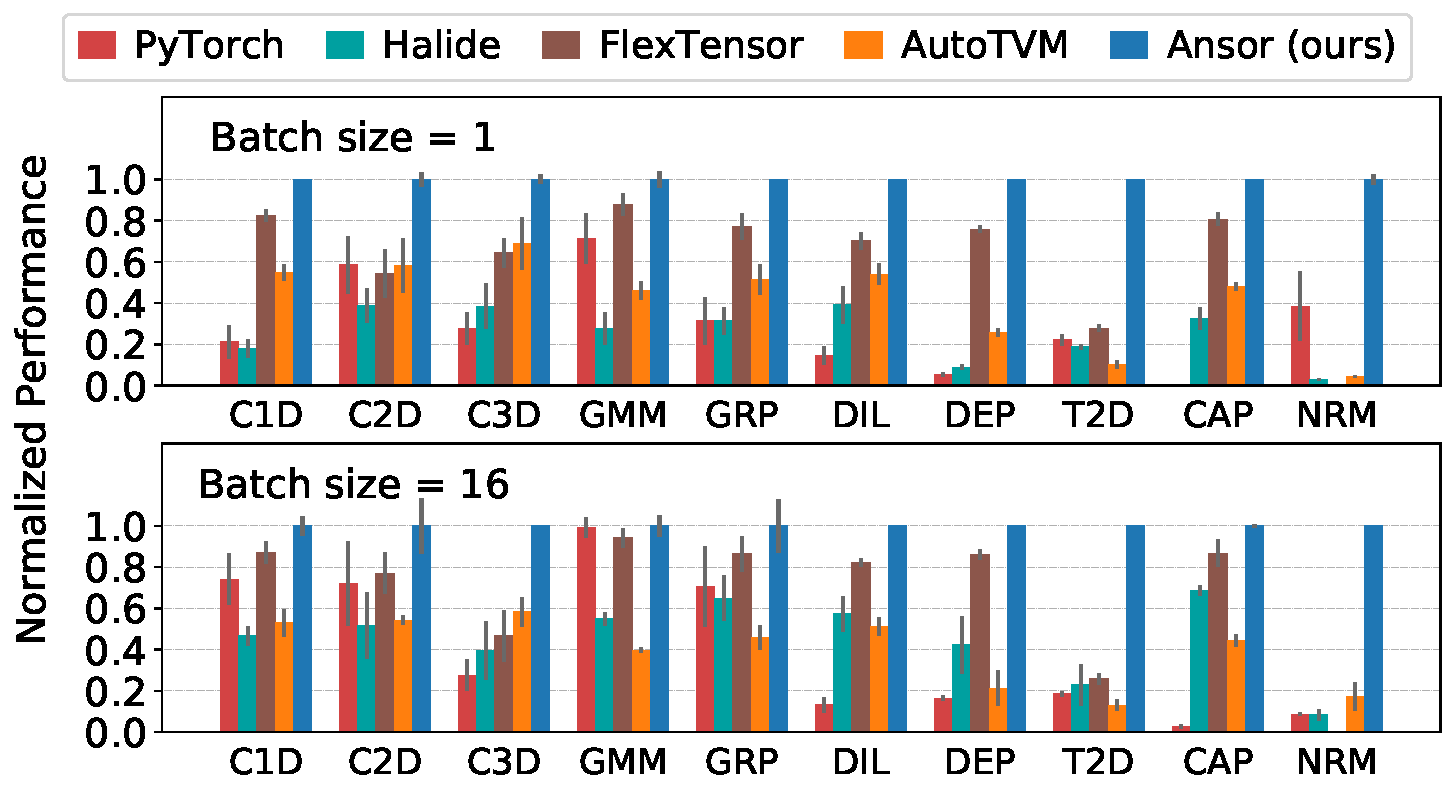
\includegraphics[width=\columnwidth]{figures/cpu-single-op.pdf}
	\precap
\caption{Single operator performance benchmark on a 20-core Intel-Platinum-8269CY. The y-axis is the throughput normalized to the best throughput for each operator.}
	\label{fig:cpu-single-op}
\end{figure}

\begin{figure}[t!]
	\centering
	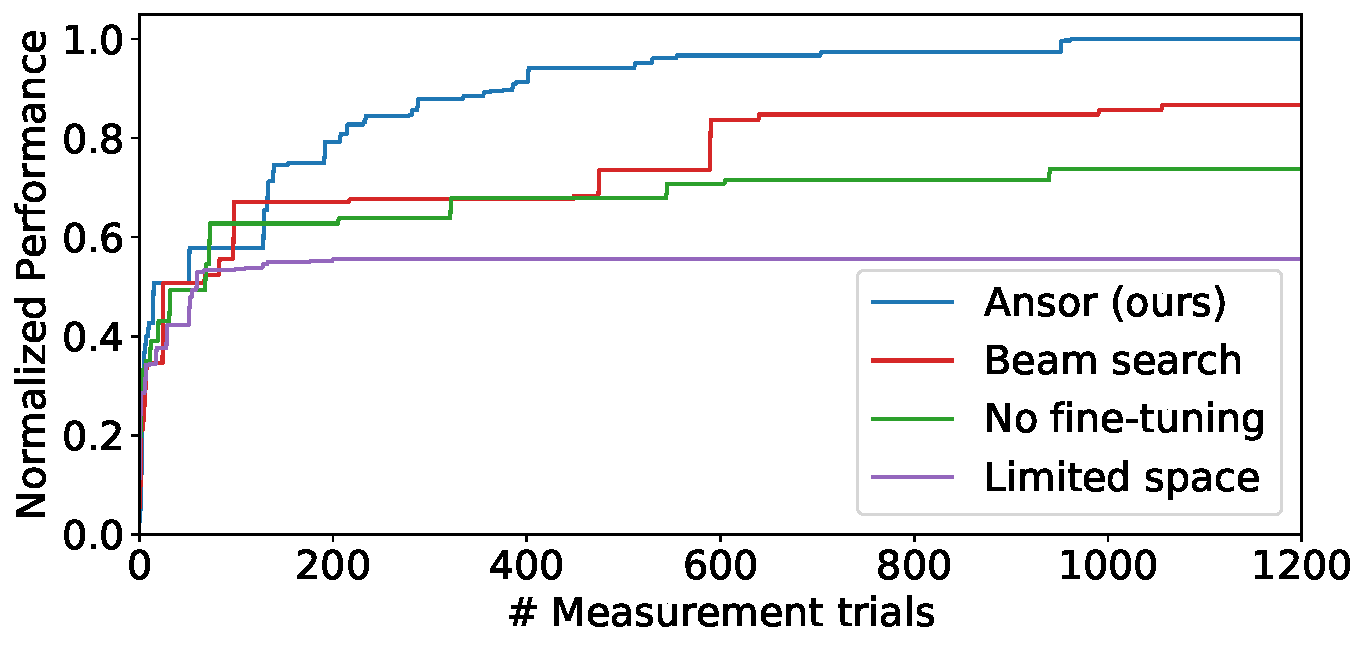
\includegraphics[width=\columnwidth]{figures/single-op-tuning-curve.pdf}
	\precap
	\caption{Ablation study of four variants of \Ansor on a convolution operator. The y-axis is the throughput relative to the throughput of the best program.}
	\postcap 
	\label{fig:cpu-op-ablation}
\end{figure}

\textbf{Ablation study.} We run four variants of \Ansor on a convolution operator and report the performance curve.
We pick the last convolution operator in ResNet-50 with batch size=16 as the test case, because its search space is sufficiently large to evaluate the search algorithms. Other operators share a similar pattern.  
In \autoref{fig:cpu-op-ablation}, each curve is the median of 5 runs.
``\Ansor (ours)'' uses all our introduced techniques.
``Beam Search'' means we prune incomplete programs with the cost model during the sampling process and do not use fine-tuning.
``No fine-tuning'' is based on ``\Ansor (ours)'' but disables fine-tuning and only relies on random sampling.
``Limited space'' is also based on ``\Ansor (ours)'' but limits the search space to make it similar to the space in existing manual templates (\textit{e.g.}, limit tiling level, innermost tile sizes, and computation location).
As demonstrated by \autoref{fig:cpu-op-ablation}, dropping either the large search space or efficient fine-tuning decreases the final performance significantly. The aggressive early pruning in ``Beam search'' throws away incomplete programs with good final performance due to inaccurate estimation.

\subsection{Subgraph Benchmark}
\label{subsec:subgraph-benchmark}

\begin{figure}[t!]
	\centering
	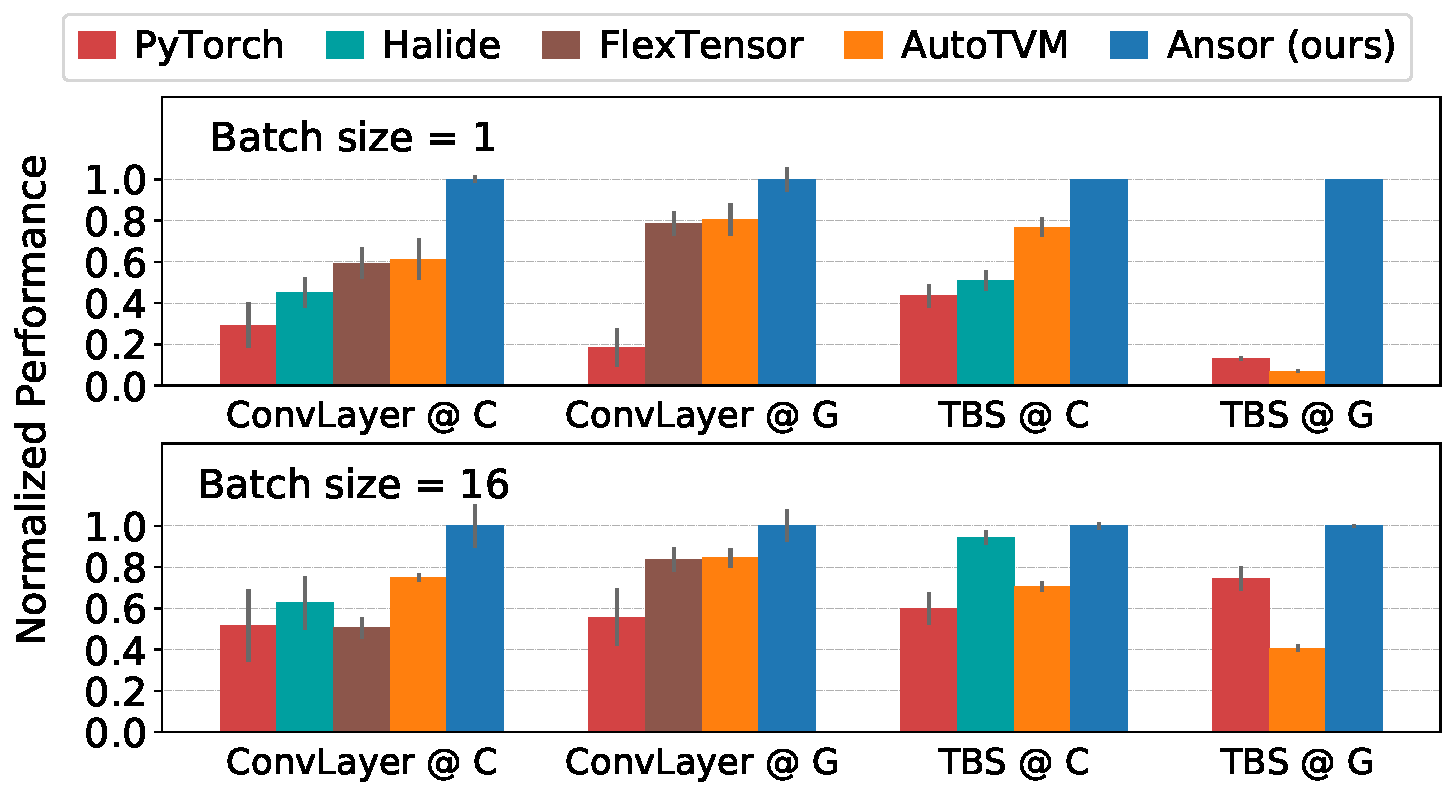
\includegraphics[width=\columnwidth]{figures/subgraph.pdf}
	\precap
	\caption{Subgraph performance benchmark on a 20-core Intel-Platinum-8269CY and an NVIDIA V100. "@C" denotes CPU results and "@G" denotes GPU results. The y-axis is the throughput normalized to the best throughput for each subgraph.}
	\postcap
	\label{fig:subgraph}
\end{figure}

We perform the subgraph benchmark on two common subgraphs in DNNs.
The ``ConvLayer'' is a subgraph consisting of 2D convolution, batch normalization \cite{ioffe2015batch}, and ReLU activation, which is a common pattern in convolutional neural networks.
The ``TBS'' is a subgraph consisting of two matrix transposes, one batch matrix multiplication, and a softmax, which is a pattern in the multi-head attention \cite{vaswani2017attention} in language models.
Similar to the single operator benchmark (\autoref{subsec:single-op-benchmark}), we select four different shape configurations and two batch sizes, run auto-tuning with up to $1,000$ measurement trails per test case, and report the normalized performance.
We use the same set of baseline frameworks and run the benchmark on the Intel CPU and the NVIDIA GPU.
We do not report the performance of Halide auto-scheduler on GPU because as of writing the paper its GPU support is still in an experimental stage. FlexTensor fails to run on complicated subgraphs like ``TBS''.

\autoref{fig:subgraph} shows that \Ansor outperforms manual libraries and other search frameworks by $1.1-14.2\times$.
\Ansor can generate high-performance programs consistently for these subgraphs on both platforms.
FlexTensor performs well for single operators but shows less advantage for subgraphs because it lacks the support of operator fusion.

\subsection{End-to-End Network Benchmark}
\label{subsec:network-benchmark}

\textbf{Workloads.}
We benchmark the end-to-end inference execution time of several DNNs, which include ResNet-50~\cite{he2016deep} and MobileNet-V2~\cite{sandler2018mobilenetv2} for image classification, 3D-ResNet-18~\cite{hara3dcnns} for action recognition, DCGAN~\cite{radford2015unsupervised} generator for image generation, and BERT~\cite{devlin2018bert} for language understanding.
We benchmark these DNNs on three hardware platforms. For the server-class Intel CPU and NVIDIA GPU, we report the results for batch size 1 and batch size 16. For the ARM CPU in the edge device, real-time feedback is typically desired, so we only report the results for batch size 1.

\textbf{Baselines and Settings.}
We include PyTorch (v1.5 with torch script), TensorFlow (v2.0 with graph mode), TensorRT (v6.0 with TensorFlow integration)~\cite{nvidia2017tensorrt}, TensorFlow Lite (V2.0), and AutoTVM as baseline frameworks. We do not include Halide auto-scheduler or FlexTensor because they lack the support of widely-used deep learning model formats (\textit{e.g.}, ONNX, TensorFlow PB) and high-level graph optimizations.
As a result, we expect that the end-to-end execution time they can achieve will be the sum of the latency of all subgraphs in a DNN.
In contract, AutoTVM can optimize a whole DNN with its manual templates and various graph-level optimizations (\textit{e.g.}, graph-level layout search~\cite{liu2019optimizing}, graph-level constant folding~\cite{roesch2019relay}) which improve the performance significantly.
\Ansor also performs layout rewrite as described in \autoref{subsec:random-sampling}.
We let both AutoTVM and \Ansor run auto-tuning until they use to $1000 \times n$ measurement trials on each DNN, where $n$ is the number of subgraphs in the DNN. This is typically enough for them to converge.
We set the objective of the task scheduler as minimizing the total latency of one DNN and generate programs for these networks one by one.
On the other hand, PyTorch, TensorFlow, TensorRT, and TensorFlow Lite are all backed by static kernel libraries (MKL-DNN on Intel CPU, CuDNN on NVIDIA GPU, and Eigen on ARM CPU) and do not need auto-tuning. We enable AVX-512 for all frameworks on the Intel CPU in this network benchmark.


\begin{figure}[t]
	\centering
	\subfloat[Intel CPU]{
		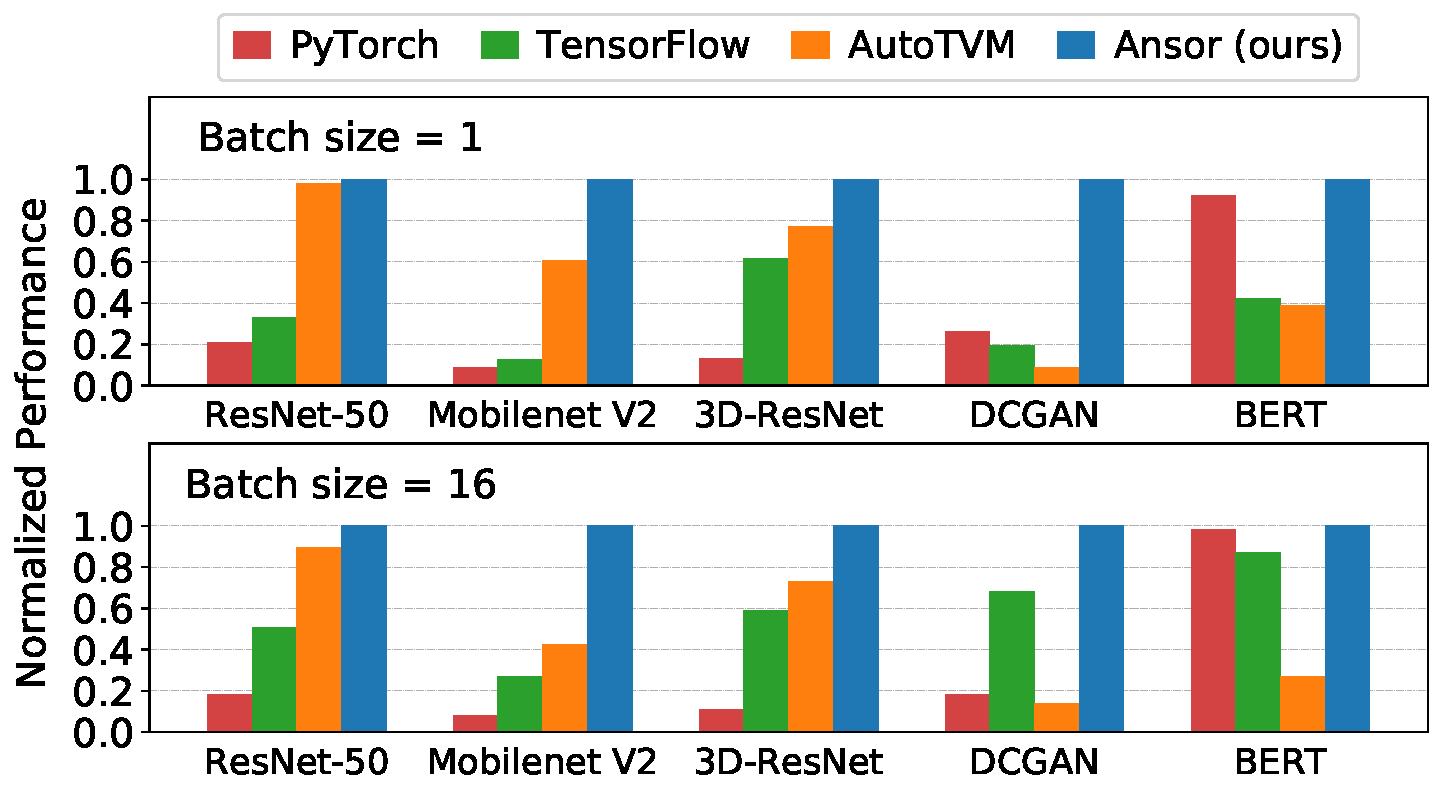
\includegraphics[width=\columnwidth]{figures/intel-network.pdf}
		\label{fig:intel-cpu-network}
	}
	
	\subfloat[NVIDIA GPU]{
		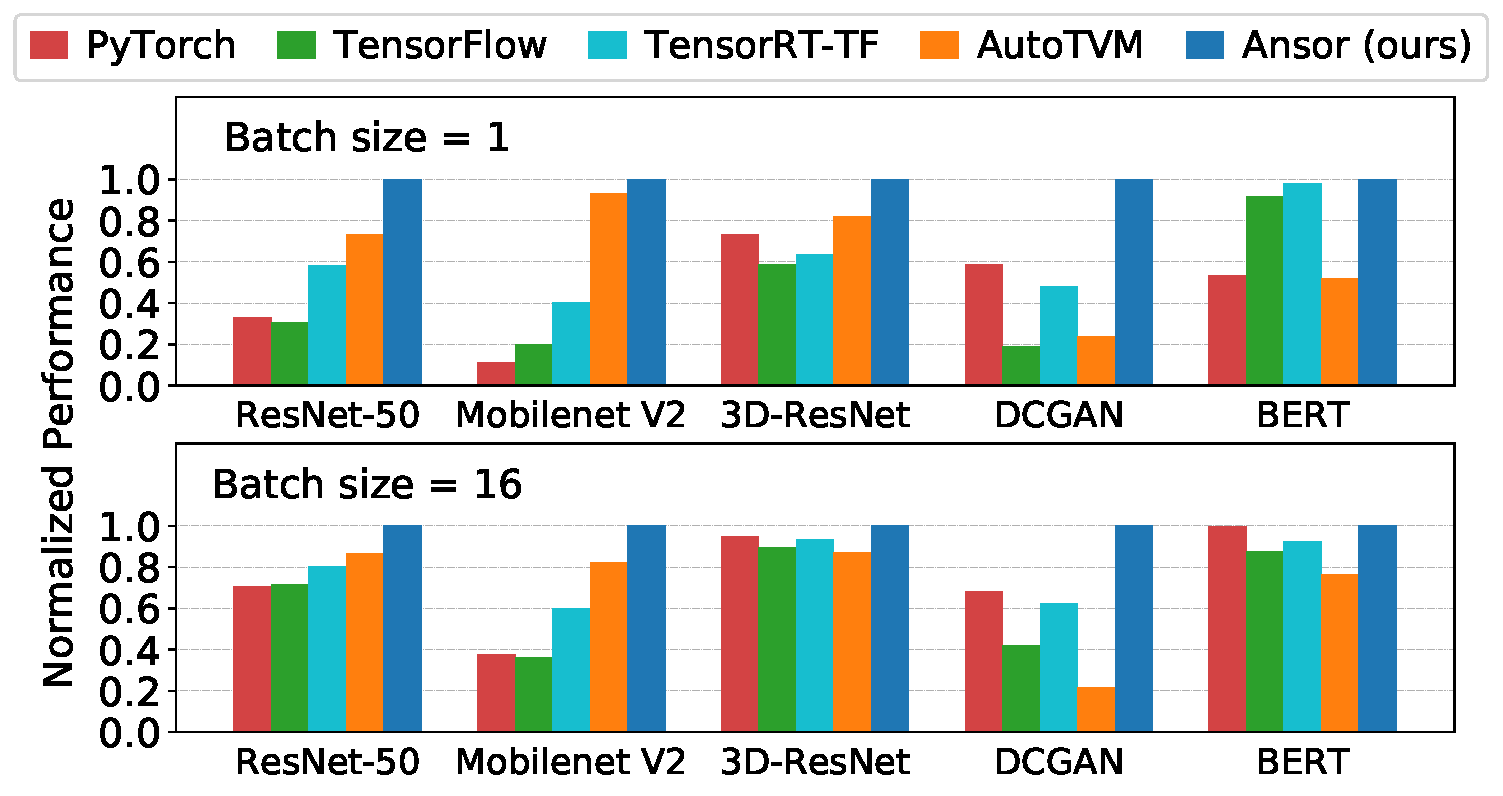
\includegraphics[width=\columnwidth]{figures/nvidia-network.pdf}
		\label{fig:nvidia-gpu-metwork}
	}
	
	\subfloat[ARM CPU]{
		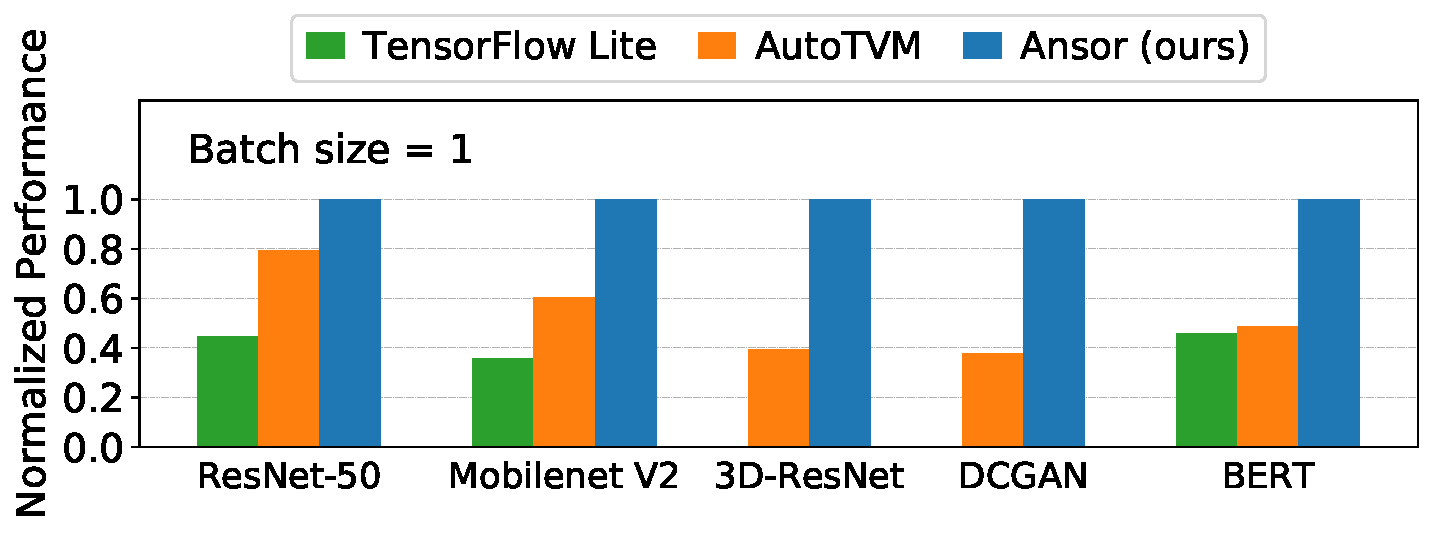
\includegraphics[width=\columnwidth]{figures/arm-network.pdf}
		\label{fig:arm-cpu-network}
	}
	\precap
	\caption{Network inference performance benchmark on three hardware platforms. The y-axis is the throughput relative to the best throughput for each network.}
	\label{fig:network-eval} 
	\postcap
\end{figure}

\textbf{Results.}
\autoref{fig:network-eval} shows the results on the Intel CPU, NVIDIA GPU and ARM CPU \footnote{3D-ResNet and DCGAN are not yet supported by TensorFlow Lite on the ARM CPU.}.
Overall, \Ansor performs the best or equally the best in all cases.
Compared with search-based AutoTVM, \Ansor matches or outperforms it in all cases with $1.0-21.8 \times$ speedup.
Compared with the best alternative, \Ansor improves the execution performance of DNNs on the Intel CPU, ARM CPU, and NVIDIA GPU by up to  $3.8\times$, $2.6\times$, and $1.7 \times$, respectively. The reason for the significant speedup on DCGAN is that DCGAN mainly consists of transposed 2D convolution (T2D), which can be well optimized by \Ansor, as shown and explained in the single operator benchmark (\autoref{subsec:single-op-benchmark}).
AutoTVM performs very well for ResNet-50 on the Intel CPU thanks to its highly-optimized templates for 2D convolution and global layout search~\cite{liu2019optimizing}. \Ansor does not run a global layout search but does rewrite the layout of weight tensors as described in \autoref{subsec:random-sampling}. \Ansor uses more levels of tiling so it packs weight tensors into more levels. The layout rewrite brings about 40\% improvement to ResNet-50 in \Ansor.
Compared with vendor-specific static libraries, \Ansor has more advantages on uncommon shapes and small batch sizes, because it is not easy to manually optimize for these cases.



\begin{figure}[t!]
	\centering
	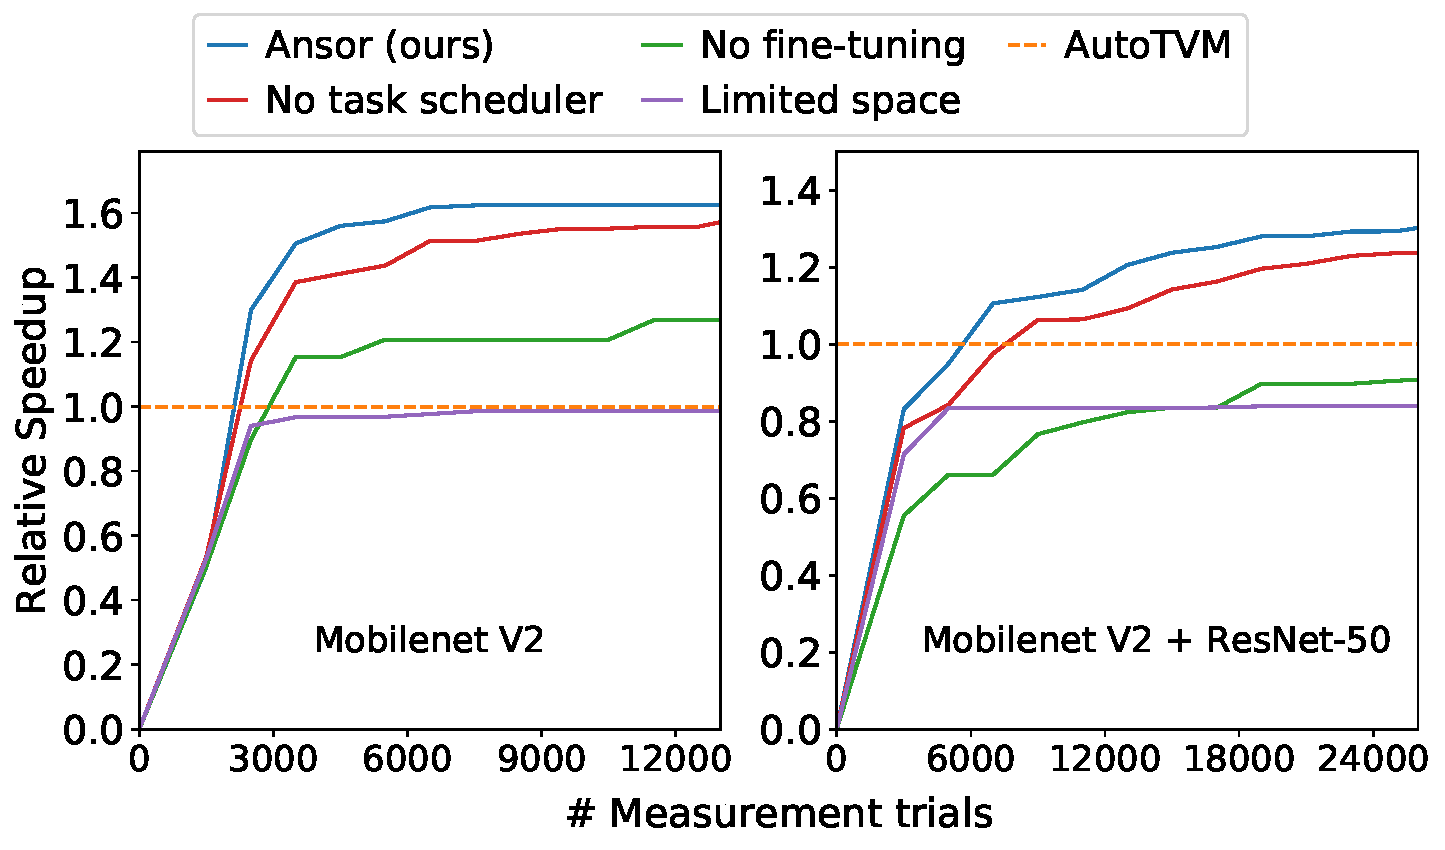
\includegraphics[width=\columnwidth]{figures/network-tuning-curve.pdf}
	\precap
	\caption{Network performance auto-tuning curve. The y-axis is the speedup relative to AutoTVM.}
	\postcap \vskip -0.5em
	\label{fig:network-tuning-curve}
\end{figure}

\textbf{Ablation study.} We run variants of \Ansor on two test cases in \autoref{fig:network-tuning-curve}. In the left figure, we run four variants of \Ansor to generate programs for a single mobilenet-V2. In the right figure, we run these variants for both mobilenet-V2 and ResNet-50.
We set the objective function of the task scheduler to be the geometric mean of speedup against AutoTVM.
As shown in \autoref{fig:network-tuning-curve}, ``No task scheduler'' means we use a round-robin strategy to allocate equal time resources to all subgraphs. ``Limited space'' is based on ``\Ansor (ours)'' but limits the search space. ``No fine-tuning'' is also based on ``\Ansor (ours)'' but disables fine-tuning and relies on random sampling only.
As can be seen in \autoref{fig:network-tuning-curve}, ``Limited space'' performs the worst in terms of the final achieved performance, proving that the best programs are not included in the limited space.
The final achieved performance can be improved by enlarging the search space, as depicted in ``No fine-tuning''.
However, in the right figure, randomly assigning tile sizes and annotations still cannot beat AutoTVM in the given time budget.
After enabling fine-tuning, ``No task scheduler'' outperforms AutoTVM in both cases.
Finally, ``\Ansor (ours)'' employs the task scheduler to prioritize performance bottlenecks (\textit{e.g.}, subgraphs contain 3x3 convolution), so it performs the best in both search efficiency and the final achieved performance.




\subsection{Search Time}

\Ansor searches efficiently and can outperform or match AutoTVM with less search time.
\Ansor slices the time and utilizes the task scheduler to simultaneously optimize all subgraphs together.
In contrast, AutoTVM and other systems do not have a task scheduler, so they generate programs for all subgraphs one by one with a predefined budget of measurement trials for each subgraph.
\Ansor saves the search time by prioritizing important subgraphs, while AutoTVM spends predefined time budget on every subgraph, which may be a waste on the unimportant subgraphs.

\autoref{table:search-time} shows the search time required for \Ansor to match the performance of AutoTVM on the Intel CPU network benchmark (\autoref{subsec:network-benchmark}). We list the search time in two metrics: number of measurements and wall-clock time. ``Number of measurements'' is a metric agnostic to the implementation of measurement and the overhead of search algorithm, while ``Wall-clock time'' takes these factors into account.
As shown in the table, \Ansor can match the performance of AutoTVM with an order of magnitude less search time.
In \autorefsuffix{table:search-time}{a} the saving in search time comes from the task scheduler, efficient fine-tuning, and comprehensive coverage of effective optimizations.
In \autorefsuffix{table:search-time}{b}, \Ansor shows more time-saving in wall-clock time. This is because \Ansor does not introduce much search overhead and has a better implementation of the measurement (on the Intel CPU, \Ansor can get accurate measurement results with fewer repetitions by explicitly flushing the cache for some tensors).
On other backends, \Ansor can match the performance of AutoTVM with a similar saving in search time.

Typically, it takes several hours for \Ansor to generate fully-optimized programs for a DNN on a single machine. This is acceptable for inference applications because it is a one-shot effort before deployment. In addition, the whole architecture of \Ansor can be parallelized very easily.

\begin{table}[t]
	\centering
	\begin{tabular}{llll}
		\hline
		& AutoTVM & Ansor & Time-saving \\
		\hline
		ResNet-50    & 21,220   & 6,403 & 3.3 $\times$   \\
		Mobilenet-V2 & 31,272   & 1,892 & 16.5 $\times$  \\
		3D-ResNet    & 5,158    & 1,927 & 2.7 $\times$   \\
		DCGAN        & 3,003    & 298   & 10.1 $\times$  \\
		BERT         & 6,220    & 496   & 12.5 $\times$  \\
		\hline
	\end{tabular}
    \vskip -0.8 em
	\caption*{(a) The number of measurements.}

	\vskip 0.8em
	\centering
	\begin{tabular}{llll}
		\hline
		             & AutoTVM & \Ansor & Time-saving       \\ \hline
		ResNet-50    & 39,250  & 4,540  & 8.6 $\times$ \\
		Mobilenet-V2 & 58,468  & 660    & 88.6 $\times$ \\
		3D-ResNet    & 7,594   & 2,296  & 3.3  $\times$ \\
		DCGAN        & 4,914   & 420    & 11.7 $\times$ \\
		BERT         & 12,007  & 266    & 45.1 $\times$ \\ \hline
	\end{tabular}
    \vskip -0.8 em
	\caption*{(b) Wall-clock time (seconds) }
	
	\caption{The number of measurements and wall-clock time used for \Ansor to match the performance of AutoTVM on the Intel CPU (batch size=1).}
	\label{table:search-time}

\end{table}


\subsection{Cost Model Evaluation}
In this subsection, we evaluate the prediction quality of the learned cost model. 
We use 25,000 programs measured during tuning ResNet-50 on the Intel CPU as the data set.
We randomly pick 20,000 programs as the training set and use the remaining 5,000 programs as the test set.
We train the cost model and let it make predictions for the test set.

\begin{figure}[t!]
	\centering
	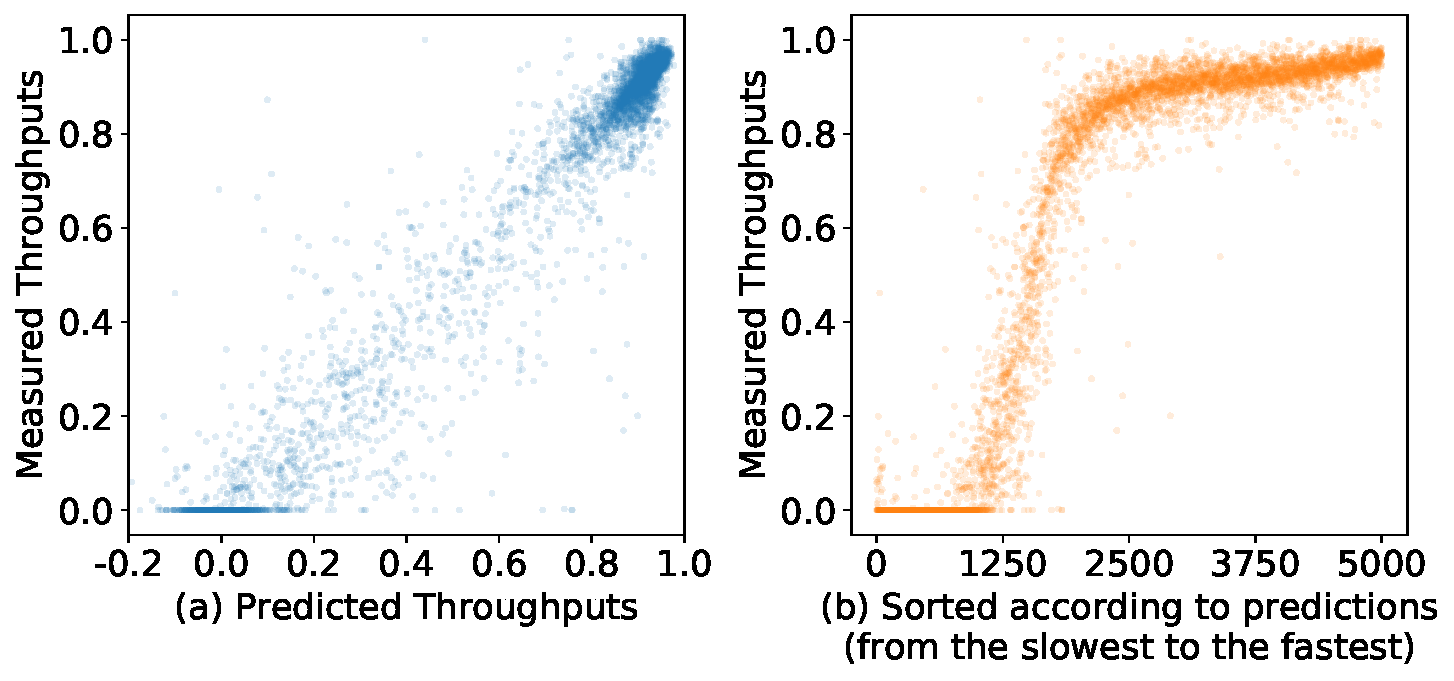
\includegraphics[width=\columnwidth]{figures/cost-model-eval.pdf}
	\precap
	\caption{Measured throughputs vs. predicted throughputs.}
	\postcap \vskip -0.5em
	\label{fig:cost-model-eval}
\end{figure}

\autoref{fig:cost-model-eval} plots the predicted throughputs vs. measured throughputs.
The measured throughputs are normalized to the best performing programs in the test set.
The predicted throughputs are the output of the model, so they can be negative.
In \autorefsuffix{fig:cost-model-eval}{a}, the points scatter around the diagonal line, meaning that the model makes accurate predictions.
The distribution is not uniform because the data set is collected during the search. Good programs have a higher probability to be chosen for measurements, so most of the programs are in the top right corner.
The points with measured throughput 0.0 are programs that are invalid or killed due to timeout during measurements.
In \autorefsuffix{fig:cost-model-eval}{b}, we sort the 5000 points according to the predictions from the slowest to the fastest, and use the relative ranking as x-axis.
So the points are distributed uniformly over x-axis. It shows the distribution of performance of the explored programs better.

The model archives  0.079 RMSE, 0.958 $R^2$ correlation, 0.851 pairwise comparison accuracy, and 0.624 recall@30 of top-30 programs (see the definition at \autoref{fn:top-k-recall-definition}) on the test set.
